\documentclass[11pt]{article}
\usepackage[a4paper,margin=2.6cm]{geometry}
\usepackage{amsmath,amssymb,amsthm}
\usepackage{graphicx}
\usepackage{xcolor}
\usepackage[colorlinks=true,linkcolor=blue!50!black]{hyperref}
\usepackage{microtype}
\graphicspath{{figs/}}
\newtheorem{lemma}{Lemma}

\title{A renormalization cell for $\int\!\!\int f_t\,g_{xx}$:\\
reducing ``does $J$ blow up?'' to one fixed point}
\author{}
\date{July 2026}

\begin{document}
\maketitle

\begin{abstract}
Maximize $J[f,g]=\int_0^1\!\!\int_{-1}^1 f_t\,g_{xx}$ over time-monotone,
$x$-convex, Lipschitz $f,g$. Single-kink competitors cap at $J=2$; a mesh
optimizer certifies $J=3.055$ and grows $\approx0.215$ per dyadic level ---
suggesting $J\sim\log N_x\to\infty$, but on two data points that a starved
optimizer would fake. We remove the extrapolation. The optimum is a
self-similar cascade of drifting curvature bands; rescaling one generation
into a co-moving unit frame turns \emph{every} generation into the same
finite ``cell'' problem acting on an environment $E$. Its fixed point
carries one number, the gain ratio $\gamma$: $\gamma\ge1$ forces
$J=+\infty$ by induction, $\gamma<1$ forces $J$ bounded. This replaces a
two-point trend with a decidable question, provable in exact arithmetic
because the cell is piecewise linear.
\end{abstract}

\section{The problem and the one obstruction}

On $Q=[-1,1]\times[0,1]$,
\begin{equation}
\sup\ J[f,g]=\int_0^1\!\!\int_{-1}^1 f_t\,g_{xx}\,\mathrm{d}x\,\mathrm{d}t,
\label{eq:J}
\end{equation}
subject to: $f(\cdot,t),g(\cdot,t)$ convex; $|f_x|,|g_x|\le1$; $f_t\ge0$,
$g_t\le0$; $f(\pm1,t)=g(\pm1,t)=0$; $f(x,1)=0$, $g(x,0)=0$. So $g_{xx}\ge0$
is a curvature measure and \eqref{eq:J} harvests $f$'s rise at $g$'s kinks.

Two budgets bound everything. \emph{Rise}, per column: $\int_0^1 f_t\,dt
=-f(x,0)\le1-|x|$. \emph{Curvature}, per slice: $\int g_{xx}(\cdot,t)\le2$
(Lipschitz). No motion creates either; it only moves them.

\paragraph{Tent cap.} Park $g$'s curvature at one fixed $x_0$: then
$J=\int_0^1 m(t)\,f_t(x_0,t)\,dt\le2(1-|x_0|)\le2$. \textbf{Any $J>2$ requires
$g$'s curvature to move.}

\section{What the optimizer does: melt (Fig.~\ref{fig:slices})}

\begin{figure}[ht]
\centering
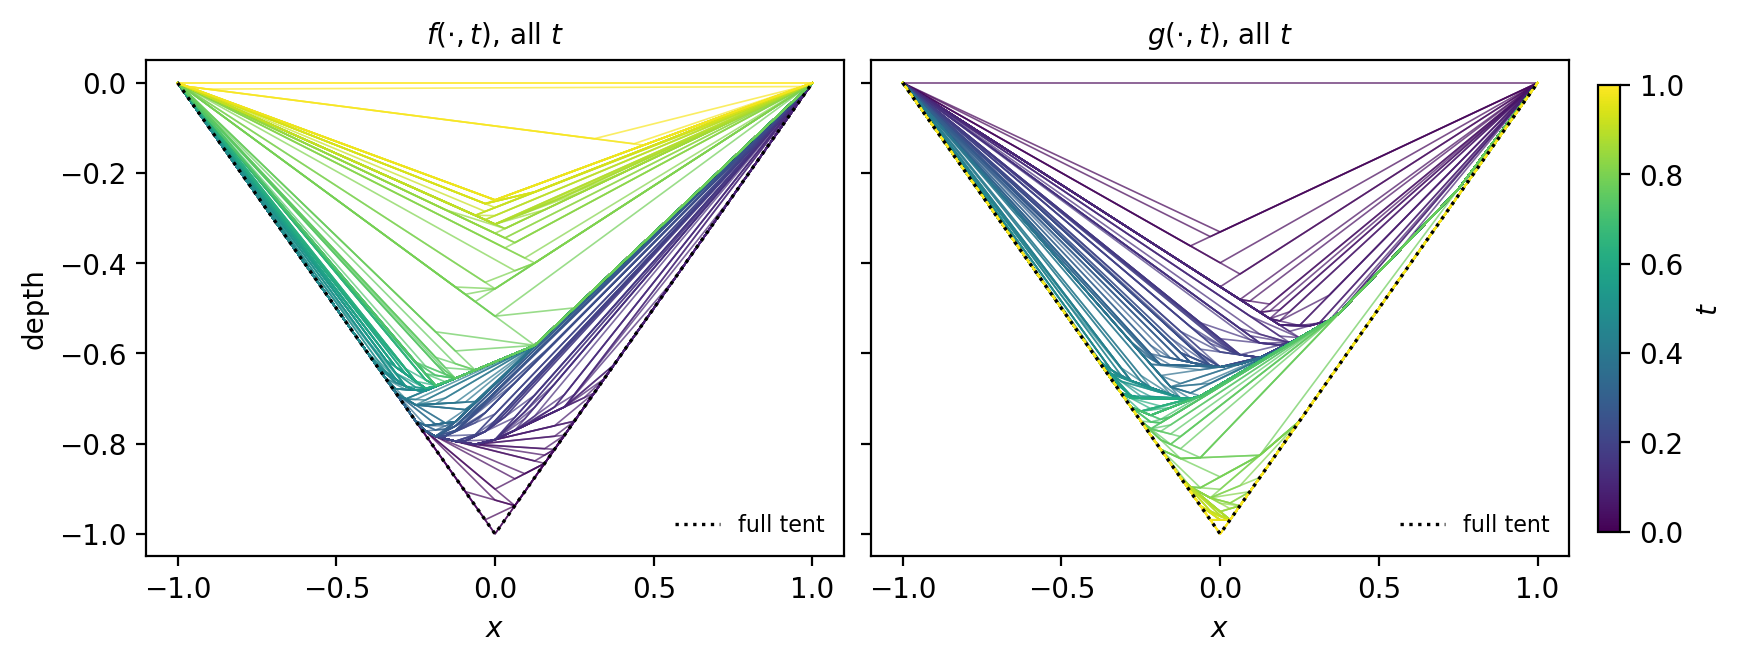
\includegraphics[width=\textwidth]{fig_slices.png}
\caption{Every time slice of the certified $J=3.055$ solution, colored by
$t$. End slices ($t{=}0$ for $f$, $t{=}1$ for $g$) are full tents; the
interior vertex \emph{melts} --- the single curvature spike spreads into a
finite-width basin whose bottom drifts off-center as $t$ runs. Arms stay at
slope $\pm1$ throughout.}
\label{fig:slices}
\end{figure}

The certified optimum keeps the end slices as full tents (rise stock) and
melts the interior: the curvature point-mass spreads into a band that
\emph{sweeps} across $x$. Same $\le2$ mass, but it now overlaps $f_t$ at
every location it visits --- and each new $x$ still holds its untapped rise
budget $1-|x|$. That is the whole engine: \textbf{sweep fixed curvature
across fresh rise budget}. It is amplification $L/w$ --- drag the curvature
far (large travel $L$), keep it thin (small width $w$).

The per-slice shape this predicts --- arms pinned at $\pm1$, the sharp vertex
melting into a widening, multi-kink basin --- is exactly what the computed
slices show, most cleanly at the best-resolved levels $k=5,6$
(Fig.~\ref{fig:realmelt}). At the tent ends the slice is a single-jump tent;
moving into the interior, the slope leaves $\pm1$ only inside a growing band,
climbing from $-1$ to $+1$ through a \emph{staircase} of several kinks --- a
distributed curvature band, not a Dirac. (The starved levels $k=7,8$ lose it:
with $M_t$ too small to resolve the moving band, the arms droop well below
$\pm1$ and the basin collapses --- the same budget effect that sends their $J$
backwards.)

\begin{figure}[ht]
\centering
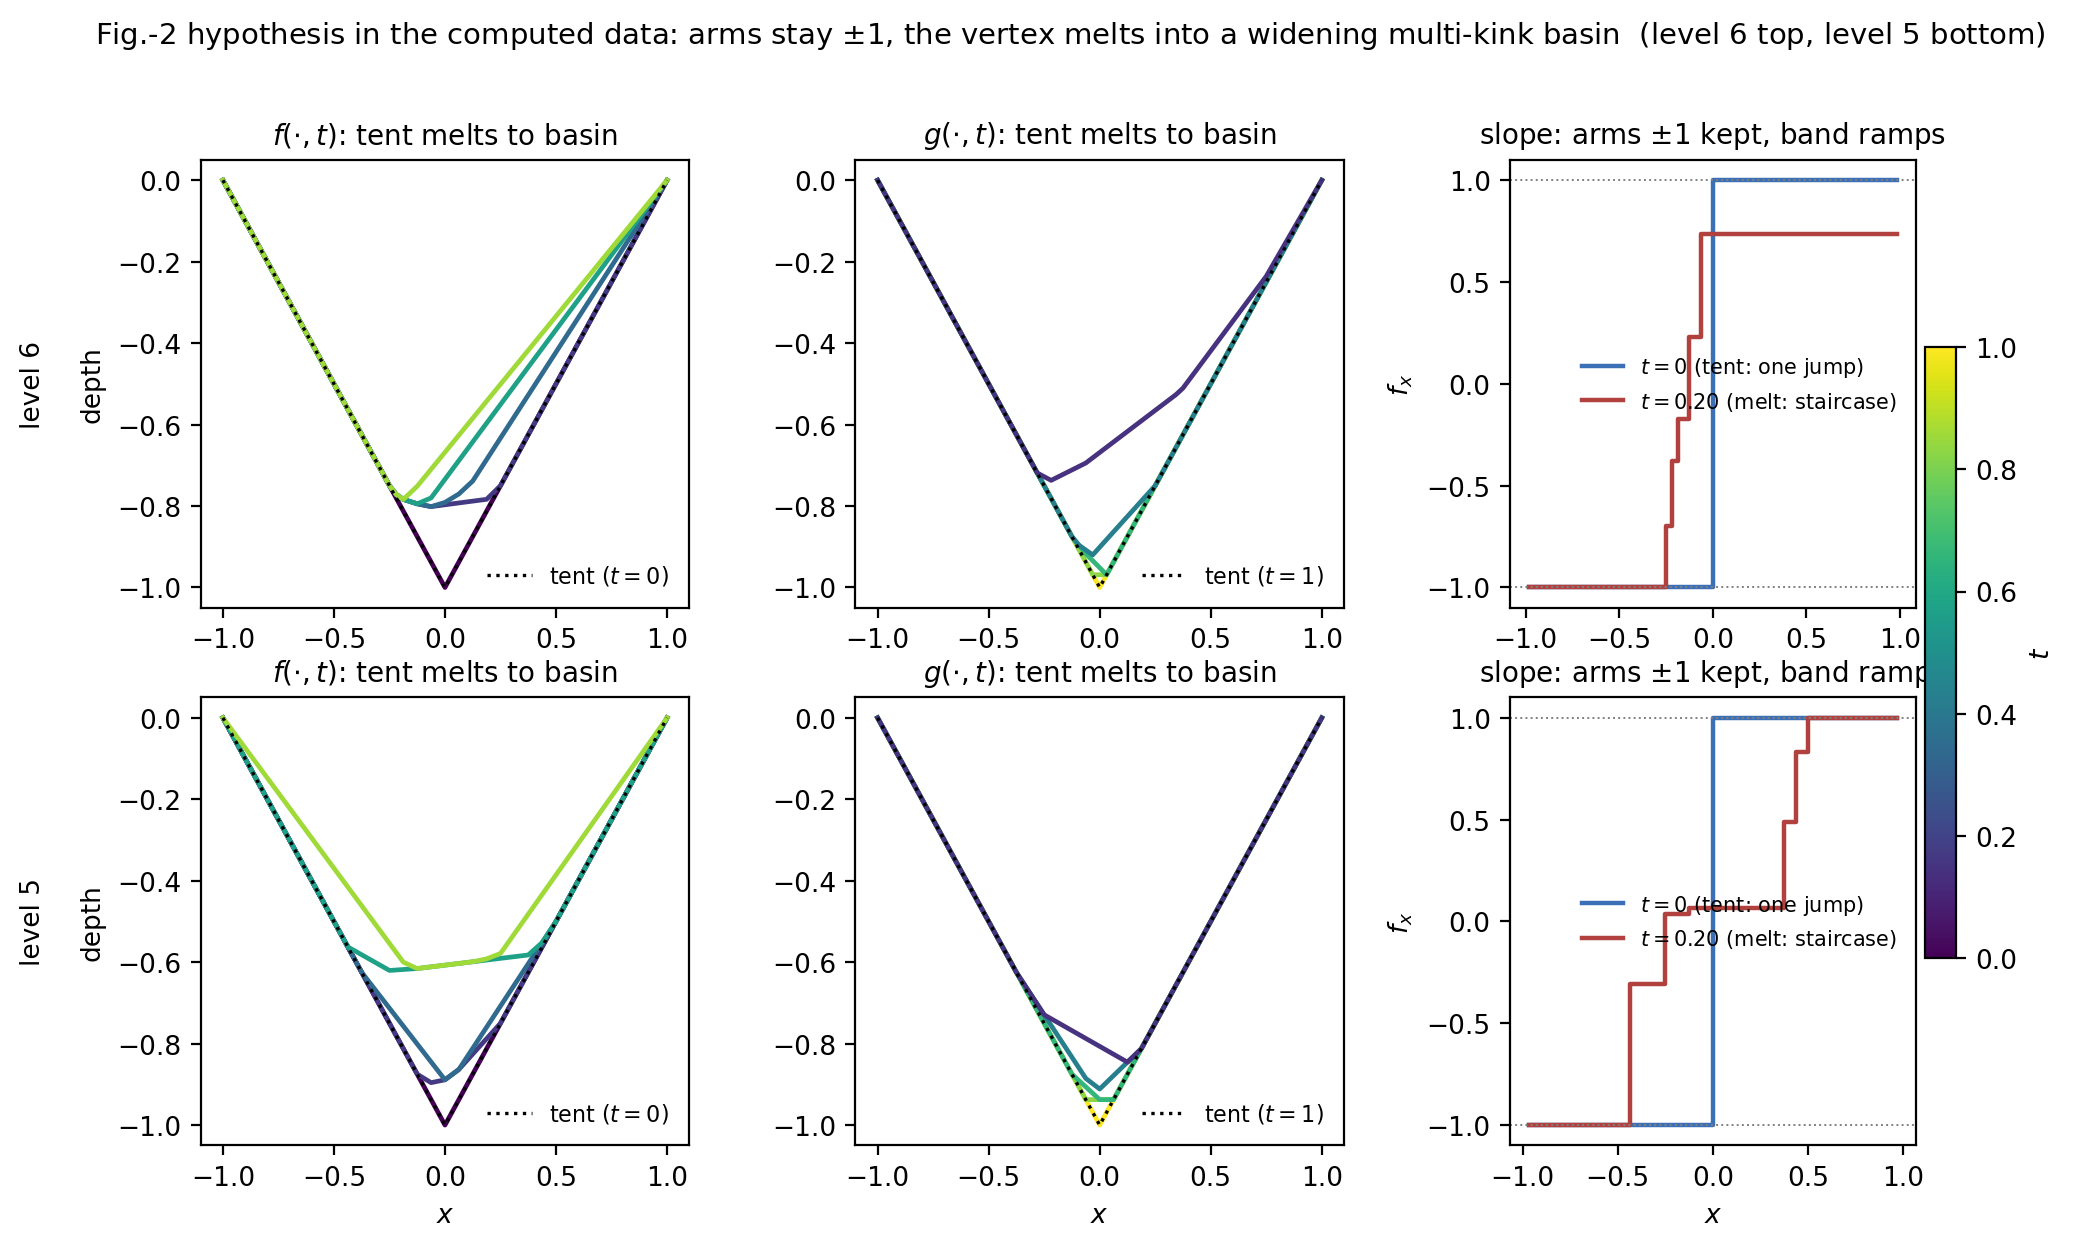
\includegraphics[width=\textwidth]{fig_realmelt.png}
\caption{The melt hypothesis in the computed cross-sections, at the levels
where it is clearest ($k=6$ top, $k=5$ bottom). Left/center: $f$ and $g$
slices colored by $t$ --- the full-depth tent (dotted) at the end time melts,
as $t$ advances, into a wide basin while the Lipschitz-$1$ arms are preserved.
Right: the slope $f_x$ --- a single $-1\!\to\!+1$ jump at the tent, versus a
multi-step staircase through a band at $t=0.20$. A melted slice is literally a
many-kink convex function.}
\label{fig:realmelt}
\end{figure}

\section{The point: one cell decides it}

Melt is self-similar: a coarse drifting basin carries a finer, faster
sub-melt, and so on --- one generation per dyadic octave
(Fig.~\ref{fig:hypo}). Whether $J\to\infty$ is exactly whether the
per-generation gain $\Delta J_k$ stays constant or decays. We turn that into
a fixed point.

\begin{figure}[ht]
\centering
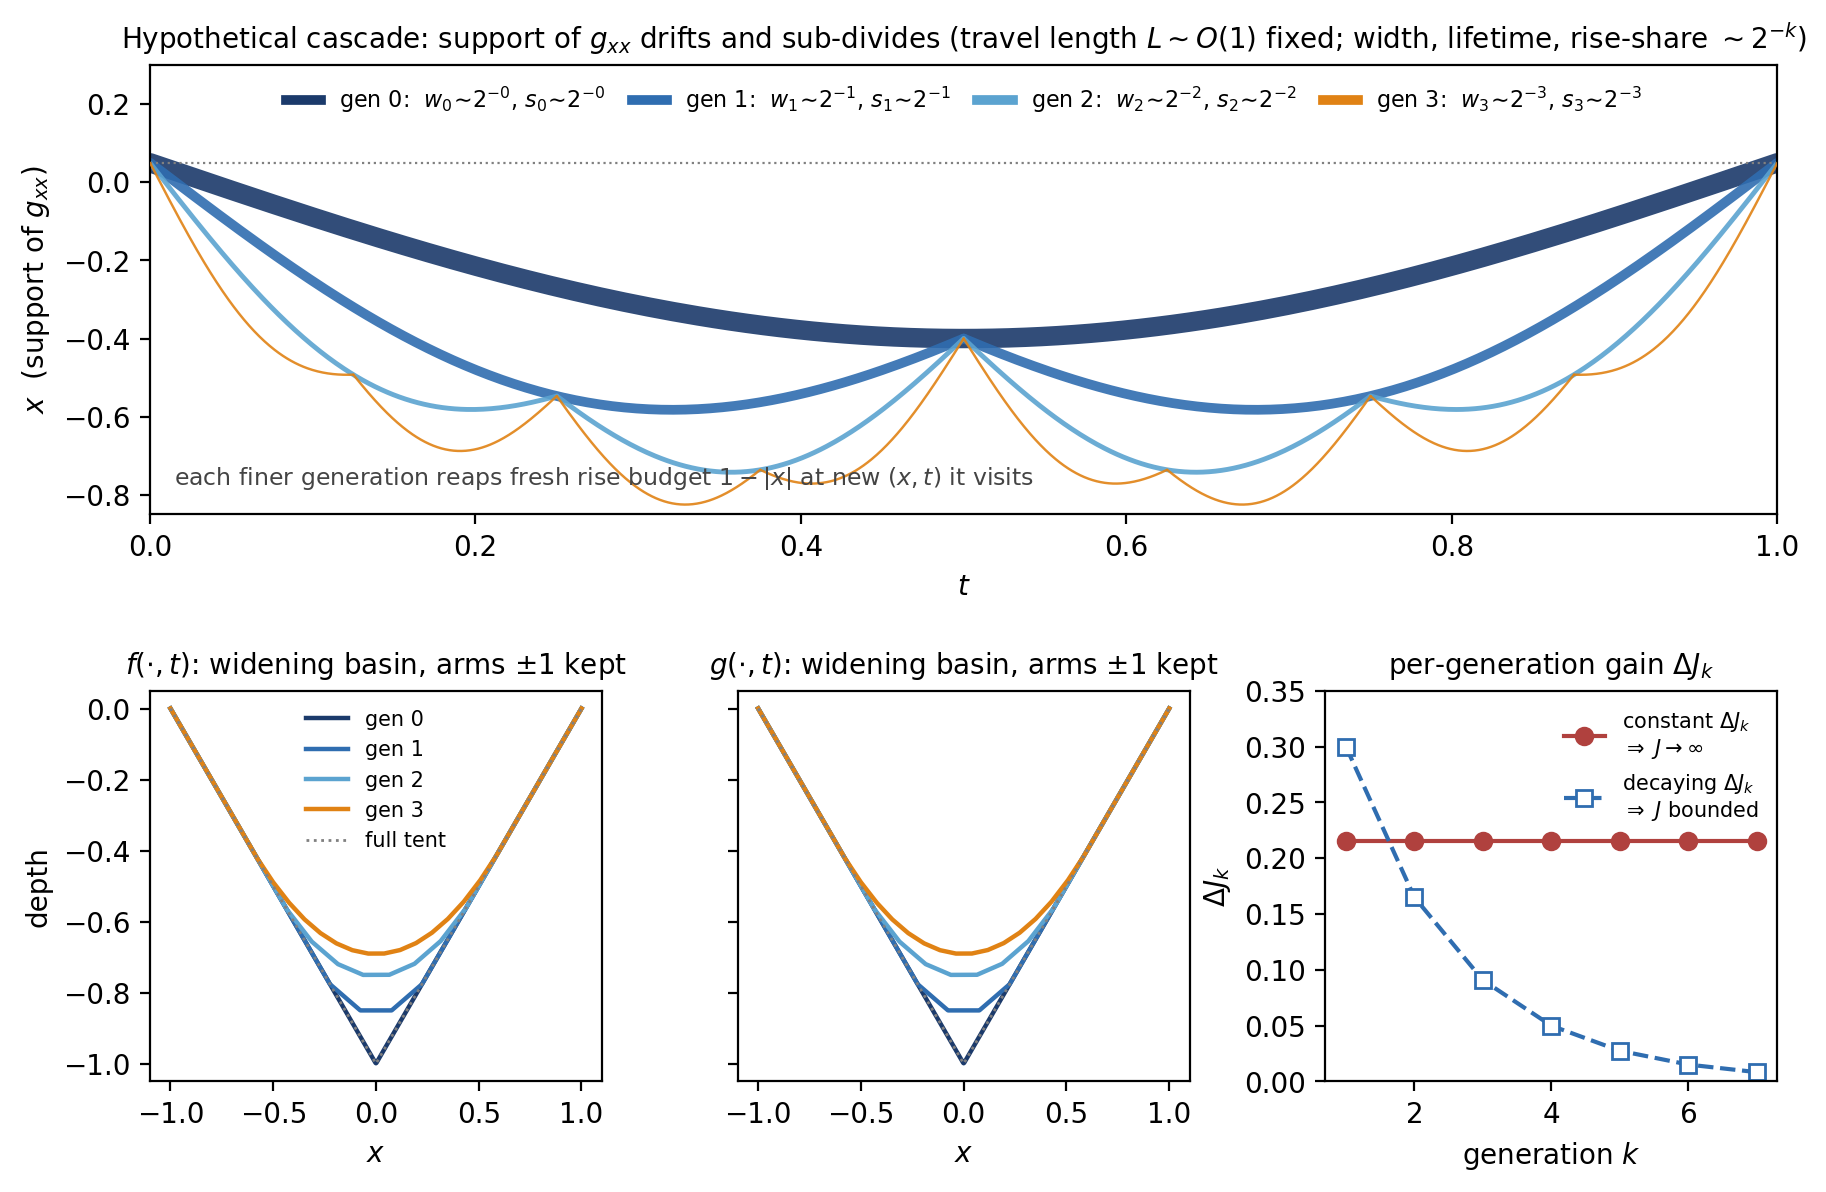
\includegraphics[width=\textwidth]{fig_hypo.png}
\caption{The conjectured cascade (schematic). Top: support of $g_{xx}$ vs
$t$ --- generation $0$ sweeps slowly over the whole interval; each finer
generation halves width $w_k$ and lifetime $s_k$, keeps an $O(1)$ travel
$L$, tiles its parent's window and rides its basin bottom. Bottom: the $f,g$
slices (widening basin, arms $\pm1$) and the decision --- constant $\Delta
J_k$ sums to $\infty$, decaying $\Delta J_k$ sums to a bound.}
\label{fig:hypo}
\end{figure}

\paragraph{Step 1 --- rescale to a unit frame.} Generation $k$ lives in a
band of width $w_k$, lifetime $s_k$, centered on a moving path $c_k(t)$. Put
$\hat x=(x-c_k(t))/w_k$, $\hat t=(t-t_k)/s_k$. In these coordinates every
generation is the \emph{same} finite object --- $O(1)$ kinks over $O(1)$
time. The cascade is one map iterated, not $n$ separate problems.

\paragraph{Step 2 --- the cell as a map on environments.} A generation does
not act in a vacuum: coarser generations leave it an \emph{environment} $E$
--- the slope slack still available near the host basin bottom, and the rise
budget not yet spent. The unit-frame problem is a map
\[
\textsc{cell}:\quad E\ \longmapsto\ \bigl(\Delta\hat J,\ E'\bigr),
\]
returning this generation's gain $\Delta\hat J$ and the environment $E'$ it
hands to its child. Solving \textsc{cell} is convex: positions are fixed by
the ansatz, weights by an LP. No nonconvex search, hence no optimizer
artifact.

\paragraph{Step 3 --- the fixed point is the answer.} Self-similarity means
the child's environment equals the parent's after rescaling: $E'=E$. At that
fixed point $E^\ast$ the gain ratio
\[
\boxed{\ \gamma=\frac{\Delta\hat J_{k+1}}{\Delta\hat J_k}\ }
\]
is a single number, and it decides \eqref{eq:J} outright:
\[
\gamma\ge1\ \Longrightarrow\ J=\sum_k\Delta J_k=+\infty
\qquad(\text{blow-up});\qquad
\gamma<1\ \Longrightarrow\ \sum_k\Delta J_k<\infty
\qquad(\text{bounded}).
\]
No extrapolation: one cell, one ratio, both directions closed.

\paragraph{Why it is a proof, not a plot.} Blow-up needs only a lower bound:
\begin{lemma}[gadget]
One explicit feasible generation, inserted in $E$, gains $\Delta J\ge c>0$
after paying its cost.
\end{lemma}
\begin{lemma}[composition]
The state after that insertion contains a rescaled copy of $E$ --- same
dimensionless data.
\end{lemma}
\noindent Together: $J\ge\sum_k c=+\infty$ by induction. The cell is
piecewise linear with finitely many kinks, so both lemmas are finite lists
of rational inequalities --- checkable exactly. Numerics only \emph{find}
the gadget and locate $E^\ast$; the induction is what proves it.

\section{What the grid already measured: $\gamma\approx1$}

The rectangular-grid optimizer gives an estimate of $\gamma$ --- but only at
the levels where it means anything. Below $N_x=17$ the solution sits exactly
on the tent cap ($\Delta J=0$: no generation yet), and the first breach
$k3\!\to\!k4$ ($\Delta J=0.625$) is the \emph{birth} of the melt, a one-time
transient, not a steady cascade octave. The ratio $\gamma=\Delta
J_{k+1}/\Delta J_k$ is therefore only defined on the two genuine
melt-refinement octaves, $k4\!\to\!k5$ and $k5\!\to\!k6$
(Fig.~\ref{fig:gamma}):
\[
\Delta J_{4\to5}=0.211,\qquad \Delta J_{5\to6}=0.219,
\qquad\Longrightarrow\qquad
\gamma=\frac{0.219}{0.211}\approx 1.04 .
\]
At the levels where the number makes sense, \textbf{$\gamma\approx1$} ---
the constant-gain, blow-up side of the dichotomy. And the bias points the
safe way: the larger increment $\Delta J_{5\to6}$ is the \emph{better}
resolved octave (it alone doubled $M_t$, $129\!\to\!257$), so if anything the
earlier $0.211$ was mildly time-starved and understated, pushing the true
$\gamma$ up, not down.

This is one ratio from two points, on exactly the quantity a starved
optimizer fakes (levels $k7,k8$, which refine $x$ but starve $t$, show
$\Delta J<0$ --- spurious ``decay''). So it \emph{suggests} $\gamma\approx1$;
it cannot settle it. That is precisely the gap the cell closes: replace this
fragile two-point ratio with $\gamma$ read at the self-reproducing
environment $E^\ast$, artifact-free.

\begin{figure}[ht]
\centering
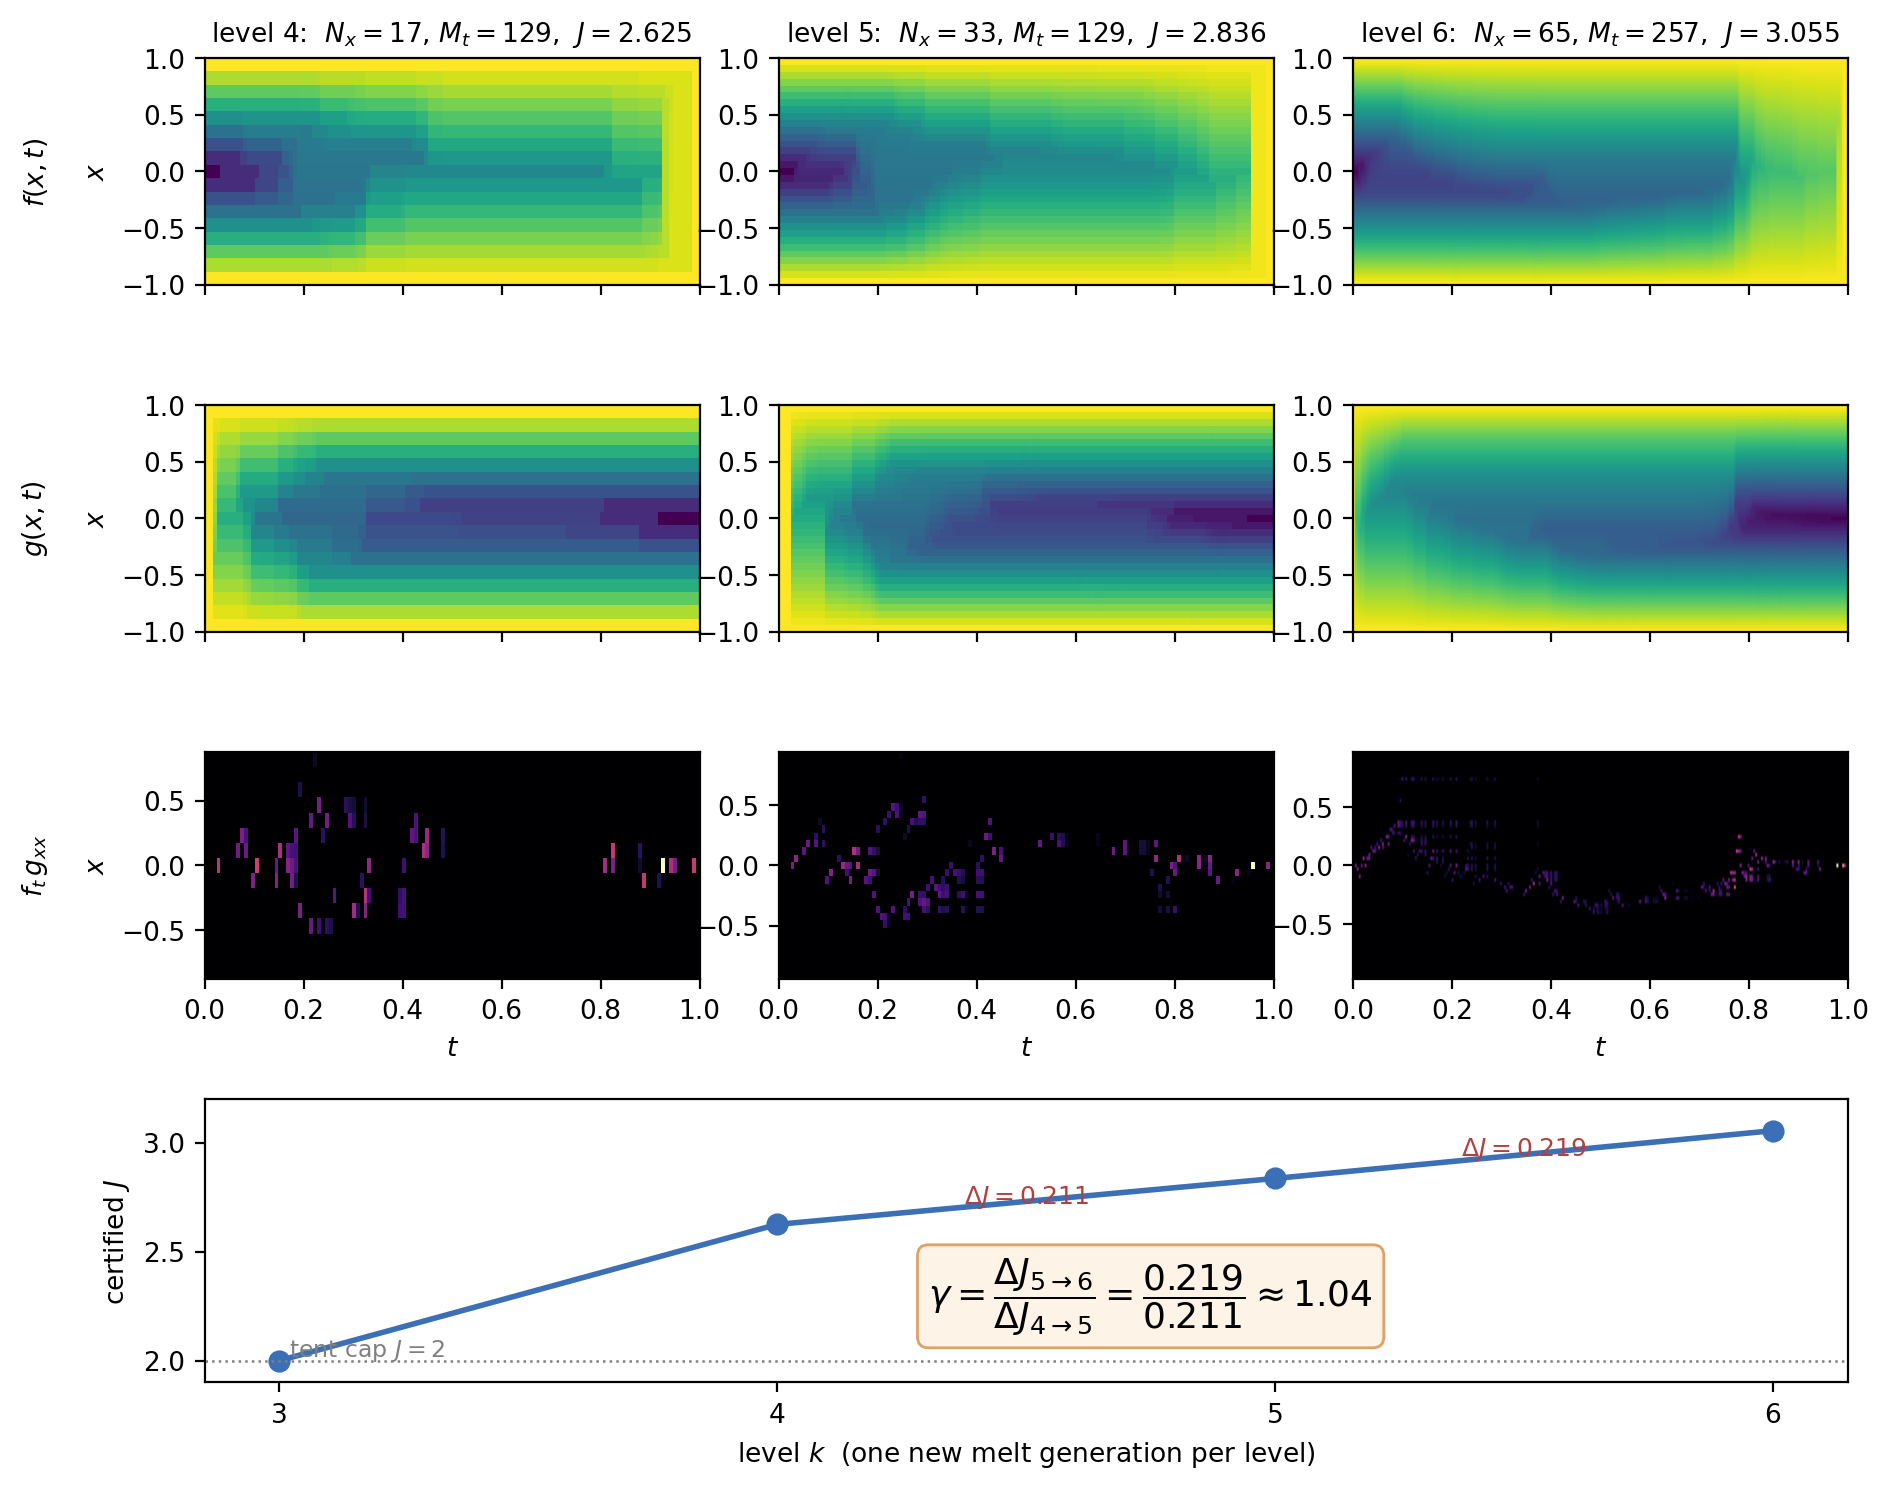
\includegraphics[width=\textwidth]{fig_gamma.png}
\caption{The melt regime $k=4,5,6$, where new generations are resolved.
Rows: $f(x,t)$, $g(x,t)$ (depth $0$ yellow to $-1$ purple), and the harvest
density $f_t\,g_{xx}$ --- whose drifting band sharpens and grows finer
sub-filaments with each level (a new generation becoming visible). Bottom:
certified $J$ vs level; the two genuine melt octaves give
$\gamma=\Delta J_{5\to6}/\Delta J_{4\to5}\approx1.04$.}
\label{fig:gamma}
\end{figure}

\section{Why nothing cheaper settles it}

\begin{itemize}
\item \textbf{Mesh:} resolving generation $k$ costs $N_x,M_t\sim2^k$ in
\emph{both} axes (starve $t$ and $J$ drops), so cost is $O(4^n)$ --- two
octaves, then dead. It also carries no composable handle: it can never
supply Lemma 2. It can only ever \emph{suggest}.
\item \textbf{Strictly self-similar cascade:} scale $x\mapsto\lambda x$,
$t\mapsto\tau t$; Lipschitz forces amplitude $\lambda$, so
$f_t\sim\lambda/\tau$, $g_{xx}\sim1/\lambda$, $dx\,dt\sim\lambda\tau$, giving
$\Delta J_k\sim\lambda^k$ --- $\gamma<1$ \emph{always}. Contracting a copy
to a point cannot blow up; a prior constructive run built exactly this and
correctly found bounded $J$, deciding nothing about the real question.
\item \textbf{The cell is the one instrument that is both} artifact-free
(convex, LP-only --- like the strict construction) \emph{and} the right
shape (drifting finite-width band, $L$ fixed while $w,s\to0$ --- like the
mesh optimum). Only anisotropic scaling ($w,s,r\sim2^{-k}$, $L\sim O(1)$)
gives $\Delta J_k\sim r_kL/w_k=$ const; the cell tests whether the one
unclosed budget --- slope slack near the basin bottom, the ``re-arm cost''
--- eats that constant. That single quantity is $\gamma$.
\end{itemize}

\paragraph{Honest edges.} A $\gamma<1$ verdict is relative to the ansatz (a
richer band could still blow up); a $\gamma\ge1$ verdict with both lemmas is
unconditional. And the environment read-off must itself pass a resolution
check --- the same starvation that faked the mesh trend can hide in it.

\end{document}
